\documentclass[a4j]{jarticle}
\usepackage{graphicx}
\usepackage[left=25truemm,right=25truemm]{geometry}

\title{画像処理 レポート}

\author{氏名: 木下直樹\\学籍番号: 09425521}

\date{提出日: 2015月11月30日}

\begin{document}
\maketitle

%%%%%%%%%%%%%%%%%%%%%%%%%%%%%%%%%%%%%%%%%%%%%%%%%%
\section{homography.cについて}
%%%%%%%%%%%%%%%%%%%%%%%%%%%%%%%%%%%%%%%%%%%%%%%%%%
homography.cのImageImageProjectionで画像を射影変換する.

3×3の行列の内, [0][0],[0][1],[1][0],[1][1]の成分は2×2の回転行列と一致する. 
[0][2],[1][2],[2][2]はそれぞれx軸y軸z軸への並行移動の値. 
[2][0],[2][1]成分は奥行きを決める.

次の行列を与えた. 

\begin{minipage}{0.5\hsize}
\begin{verbatim}

 double a[][3]={
     .866 , -.5  ,  160,
     .5   , .866 , -300,
     0    , 0    , 1
  };

\end{verbatim}
\end{minipage}

\begin{minipage}{0.5\hsize}
\begin{verbatim}

  double b[][3]={
     .866 , -.5  ,  160,
     .5   , .866 , -300,
     -.001, 0    , 1
  };

\end{verbatim}
\end{minipage}

行列a,bでは[2][0]成分の値が異なる. 実際に実行した結果は以下である. 

\begin{figure}[htbp]
\begin{tabular}{ccc}
\begin{minipage}{0.4\hsize}
\center
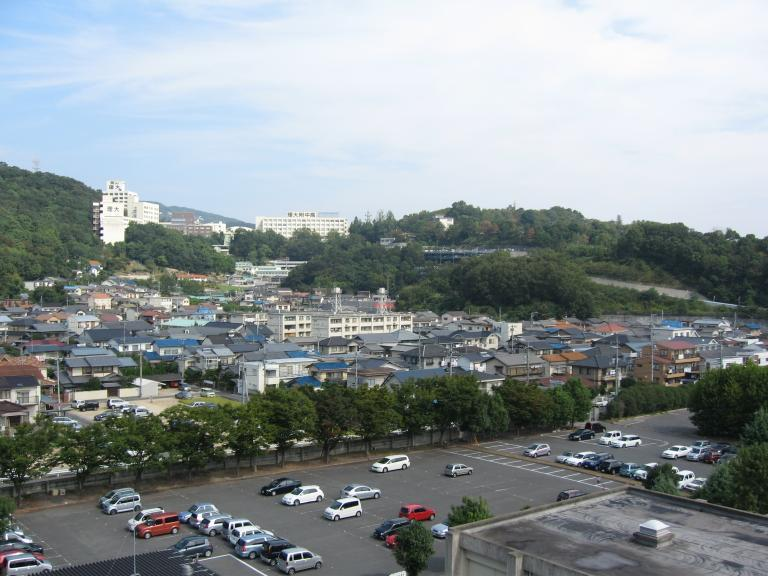
\includegraphics[bb=0 0 768 576,scale=.2]{0.jpg}
\caption{変換前の元画像}
\end{minipage}
\begin{minipage}{0.3\hsize}
\center
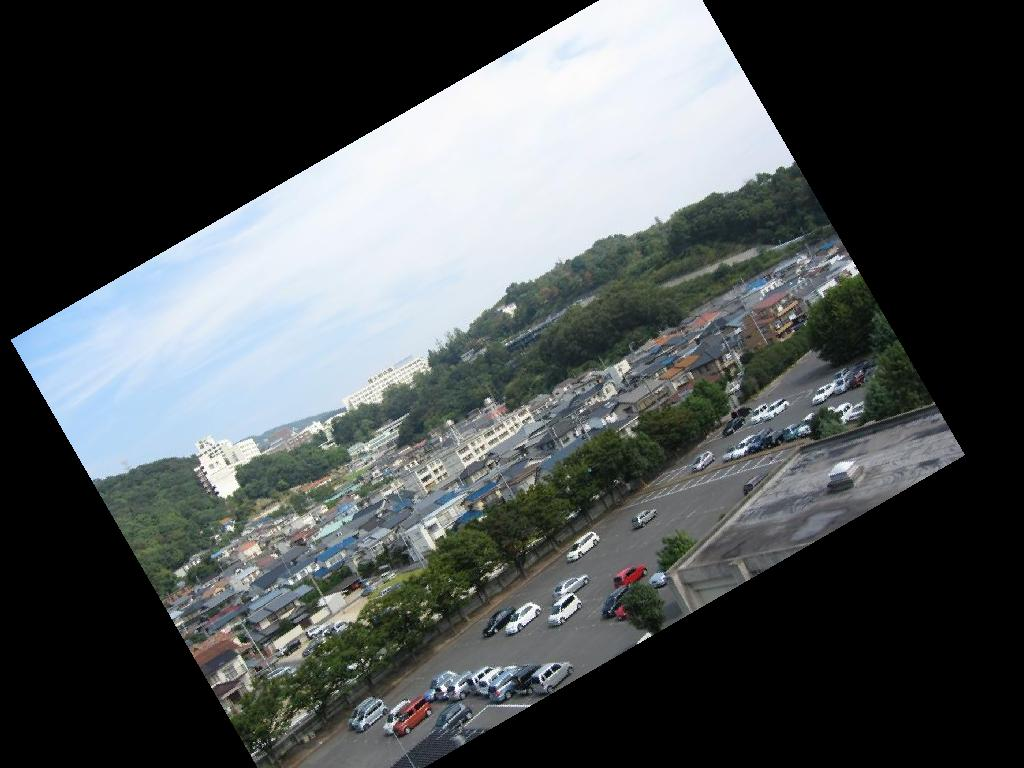
\includegraphics[bb=0 0 1024 768,scale=.13]{outa.jpg}
\caption{行列aでの変換}
\end{minipage}
\begin{minipage}{0.3\hsize}
\center
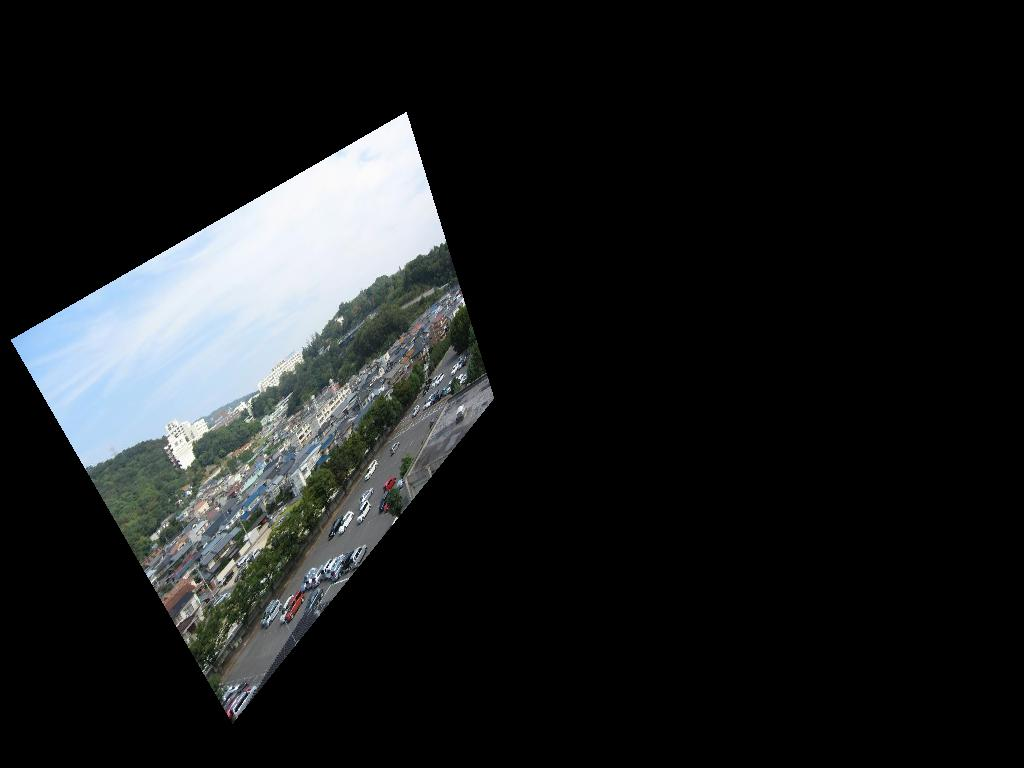
\includegraphics[bb=0 0 1024 768,scale=.13]{outb.jpg}
\caption{行列bでの変換}
\end{minipage}
\end{tabular}
\end{figure}

どちらも画像の左上の位置は一致しており, 左上の点がy軸上の点として, xz平面で反時計回りに回転したような画像の変形になっている. 

\newpage
%%%%%%%%%%%%%%%%%%%%%%%%%%%%%%%%%%%%%%%%%%%%%%%%%%
\section{pano0.cについて}
%%%%%%%%%%%%%%%%%%%%%%%%%%%%%%%%%%%%%%%%%%%%%%%%%%
このプログラムでは, 同一視点から撮影された遠景の画像を射影変換によって重ね合わせ, 1枚のパノラマ画像のような画像を作り出すものである. 以下の行列m0d,m1dで変換した元画像と生成画像を示す. 

\begin{minipage}{0.5\hsize}
\begin{verbatim}

    double m0d[][3]={
      1,0,-100,
      0,1,-100,
      0,0,1
    };
\end{verbatim}
\end{minipage}
\begin{minipage}{0.5\hsize}
\begin{verbatim}

    double m1d[][3]={
       0.980063, 0.155844, -15.090362,
      -0.055756, 1.153389, -109.259360,
      -0.000139, 0.000316, 0.982279
    };
\end{verbatim}
\end{minipage}

\begin{figure}[htbp]
\begin{tabular}{ccc}
\begin{minipage}{0.3\hsize}
\center
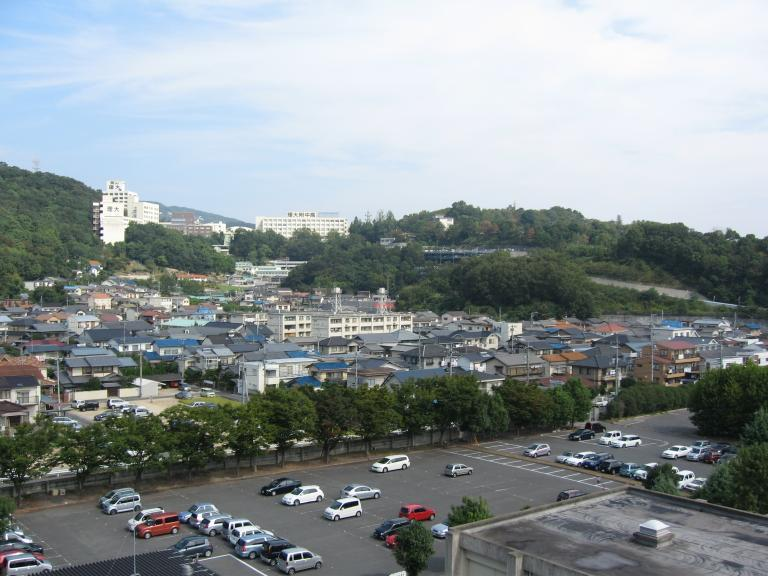
\includegraphics[bb=0 0 768 576,scale=.15]{0.jpg}
\caption{行列m0dで変換する元画像1}
\end{minipage}
\begin{minipage}{0.3\hsize}
\center
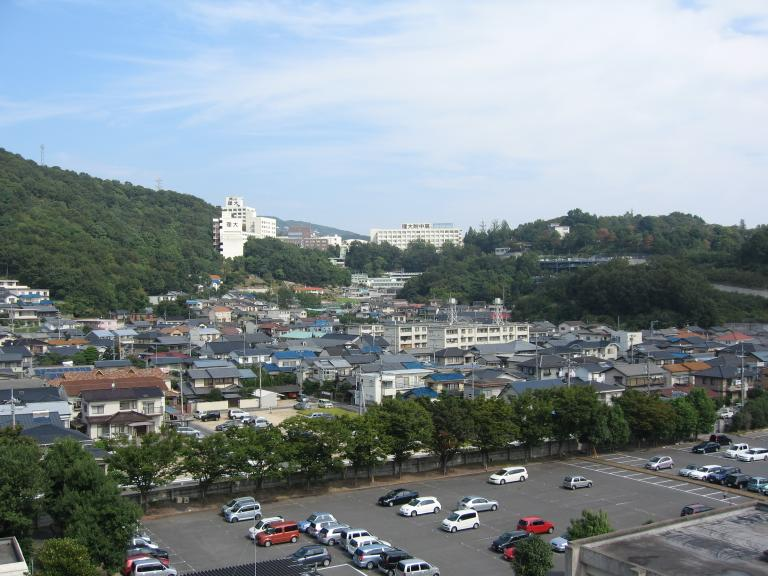
\includegraphics[bb=0 0 768 576,scale=.15]{1.jpg}
\caption{行列m1dで変換する元画像2}
\end{minipage}
\begin{minipage}{0.4\hsize}
\center
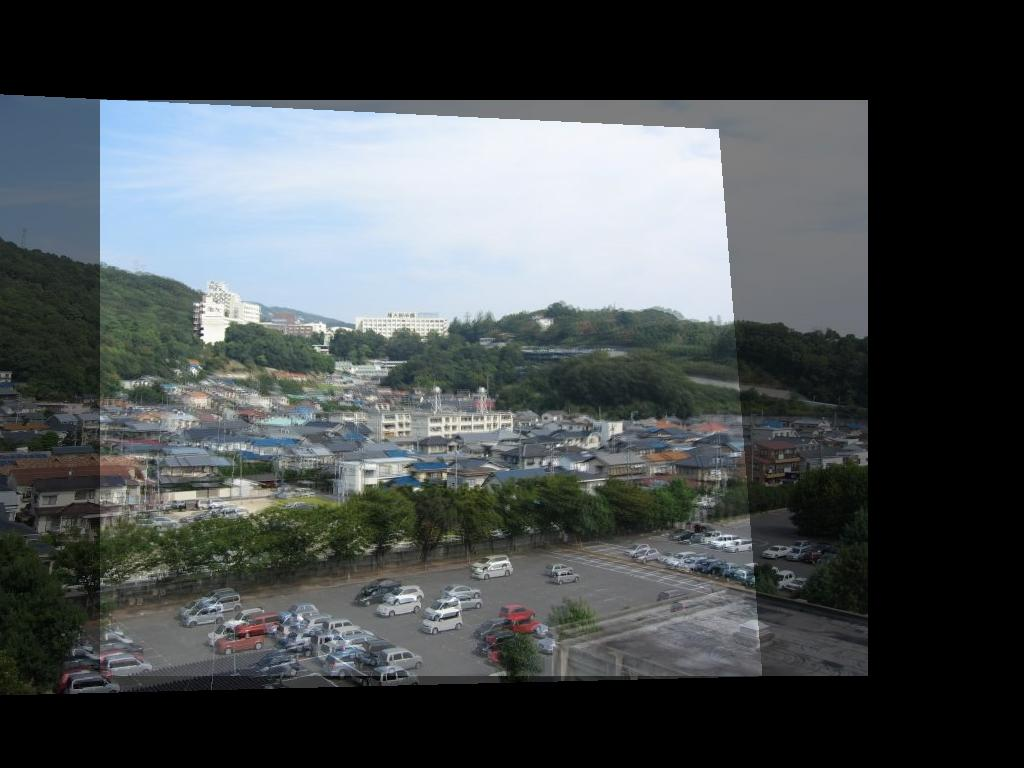
\includegraphics[bb=0 0 1024 768,scale=.15]{panoout.jpg}
\caption{生成したパノラマ画像}
\end{minipage}
\end{tabular}
\end{figure}

%%%%%%%%%%%%%%%%%%%%%%%%%%%%%%%%%%%%%%%%%%%%%%%%%%
\section{pano0.cの改良}
%%%%%%%%%%%%%%%%%%%%%%%%%%%%%%%%%%%%%%%%%%%%%%%%%%
pano0.cではm0dの値が変わると二枚の画像が上手く重ねられない. 
そこでm1dの値はm0dと以下の行列m10の行列積をとるようにする.
\begin{verbatim}

    double m10[][3]={
      0.980063, 0.155844, 98.500361,
      -0.055756, 1.153389, 0.503900,
      -0.000139, 0.000316, 1
    }

\end{verbatim}

以下の関数で行列積を計算した. 
\begin{verbatim}

void mult33(double a[3][3],double b[3][3], double c[3][3]){
  int i,j,k;
  for(i=0;i<3;i++) {
    for(j=0;j<3;j++) {
      for(k=0;k<3;k++) {
	a[i][j]+=b[i][k]*c[k][j];
      }
    }
  }
}

\end{verbatim}

\end{document}
